Eines der Ziele dieses Projekts war die praktische Umsetzung an einem Beispiel. Als Beispielobjekt wurde ein innenliegendes Treppenhaus gewählt. \\\\
Der Raspberry Pi wurde am oberen Ende der Treppe installiert und der LED-Streifen verlief an einer Seite der Treppe nach unten. Jeweils am Ende des Streifens wurde ein Bewegungssensor angebracht. Die Kamera wurde im oberen Bereich an der Wand befestigt, von wo aus ein guter Blickwinkel auf die Treppe geboten war. Als FTP-Server wurde ein vorhandener NAS eingesetzt.\\\\
Bis zum Aufbau wurden die einzelnen Komponenten über ein Experimentierboard verbunden. Da dies sehr fehleranfällig war, wurde eine kleine Platine entworfen. Diese sollte ein Steckfeld darstellen, auf dem die Komponenten leicht und sicher verbunden werden können. Der Entwurf wurde mit der Software EAGLE angefertig, welche auch in professionellen Bereichen eingesetzt wird. Sie bietet die Möglichkeit zum Erstellung von komplexen Schaltungen und automatischem Routing von Platinen. 
\begin{figure}[h]
	\begin{minipage}{\textwidth}
		\centering
		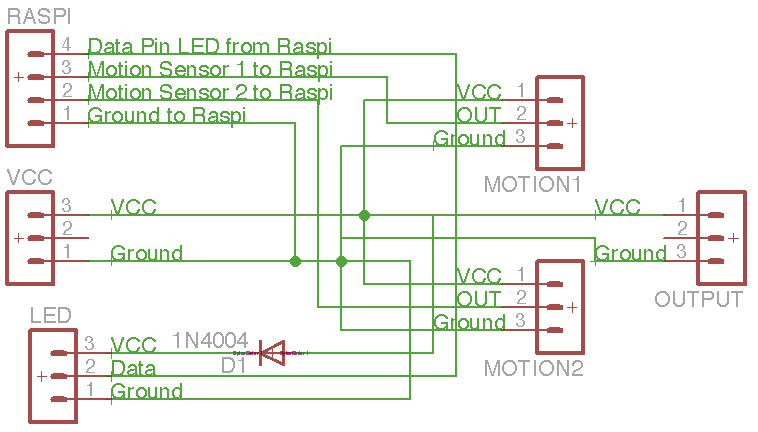
\includegraphics[width=0.8\textwidth]{./data/eagle.png}
		\caption{Schaltplan der Steckplatine}
	\end{minipage}
\end{figure}

Das zugehörige Layout und Bilder der Platine befinden sich im Anhang.
\paragraph{Fazit} Die Anwendung war einige Tage in Betrieb und funktionierte gut. Es wurden alle Funktionen getestet. Die Benachrichtigung auf das Smartphone funktionierte problemlos und innerhalb des Netzwerks konnte direkt zum Live-View gewechselt werden. 